\documentclass[tikz,border=10pt]{standalone}

\usetikzlibrary{
    positioning,
    arrows.meta,
    shapes,
    fit
}

\begin{document}

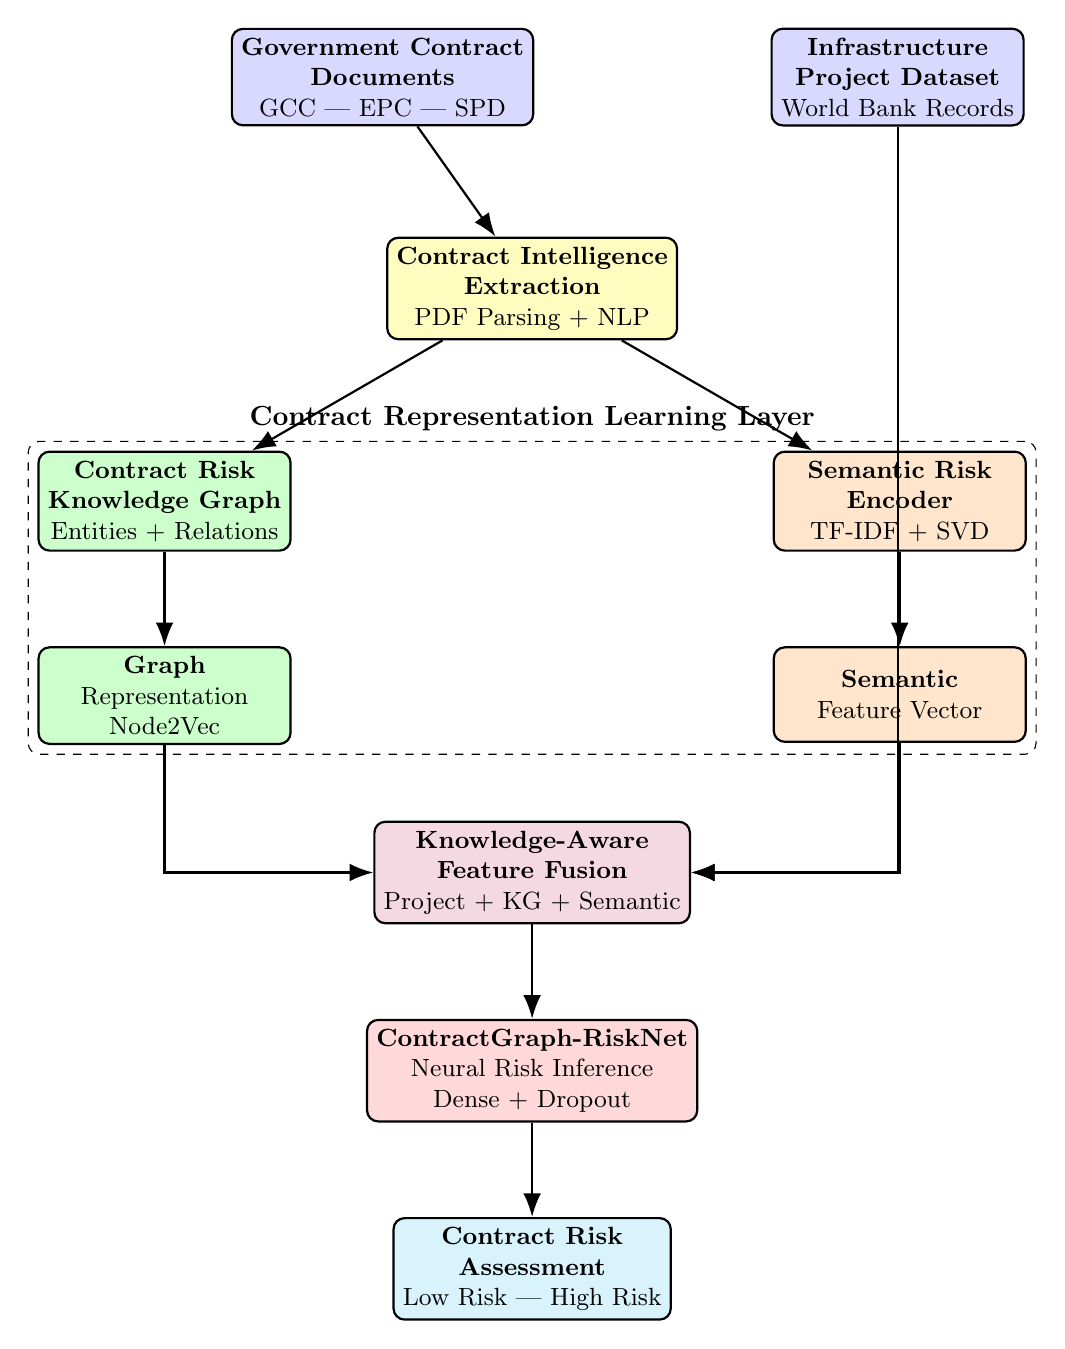
\begin{tikzpicture}
[
    font=\small,
    block/.style={
        rectangle,
        rounded corners,
        draw=black,
        thick,
        align=center,
        minimum width=3.2cm,
        minimum height=1.2cm
    },
    arrow/.style={
        -{Latex[length=3mm]},
        thick
    }
]


% =====================
% INPUT LAYER
% =====================

\node[
block,
fill=blue!15
]
(contracts)
{
\textbf{Government Contract}\\
\textbf{Documents}\\
GCC | EPC | SPD
};


\node[
block,
fill=blue!15,
right=3cm of contracts
]
(projects)
{
\textbf{Infrastructure}\\
\textbf{Project Dataset}\\
World Bank Records
};



% =====================
% EXTRACTION
% =====================

\node[
block,
fill=yellow!25,
below=1.4cm of contracts,
xshift=1.9cm
]
(extract)
{
\textbf{Contract Intelligence}\\
\textbf{Extraction}\\
PDF Parsing + NLP
};



% =====================
% REPRESENTATION
% =====================

\node[
block,
fill=green!20,
below left=1.4cm and 1.2cm of extract
]
(kg)
{
\textbf{Contract Risk}\\
\textbf{Knowledge Graph}\\
Entities + Relations
};


\node[
block,
fill=orange!20,
below right=1.4cm and 1.2cm of extract
]
(semantic)
{
\textbf{Semantic Risk}\\
\textbf{Encoder}\\
TF-IDF + SVD
};



% =====================
% EMBEDDINGS
% =====================

\node[
block,
fill=green!20,
below=1.2cm of kg
]
(node2vec)
{
\textbf{Graph}\\
Representation\\
Node2Vec
};


\node[
block,
fill=orange!20,
below=1.2cm of semantic
]
(semvec)
{
\textbf{Semantic}\\
Feature Vector
};



% =====================
% FUSION
% =====================

\node[
block,
fill=purple!15,
below=1.5cm of extract,
yshift=-4.6cm
]
(fusion)
{
\textbf{Knowledge-Aware}\\
\textbf{Feature Fusion}\\
Project + KG + Semantic
};



% =====================
% MODEL
% =====================

\node[
block,
fill=red!15,
below=1.2cm of fusion
]
(model)
{
\textbf{ContractGraph-RiskNet}\\
Neural Risk Inference\\
Dense + Dropout
};



% =====================
% OUTPUT
% =====================

\node[
block,
fill=cyan!15,
below=1.2cm of model
]
(output)
{
\textbf{Contract Risk}\\
\textbf{Assessment}\\
Low Risk | High Risk
};



% =====================
% CONNECTIONS
% =====================


\draw[arrow]
(contracts)
--
(extract);


\draw[arrow]
(extract)
--
(kg);


\draw[arrow]
(extract)
--
(semantic);


\draw[arrow]
(kg)
--
(node2vec);


\draw[arrow]
(semantic)
--
(semvec);


\draw[arrow]
(node2vec)
|- 
(fusion);


\draw[arrow]
(semvec)
|-
(fusion);


\draw[arrow]
(projects)
|-
(fusion);


\draw[arrow]
(fusion)
--
(model);


\draw[arrow]
(model)
--
(output);



% =====================
% TITLE BOX
% =====================

\node[
draw,
dashed,
rounded corners,
fit=(kg)(semantic)(node2vec)(semvec),
label={[font=\bfseries]above:Contract Representation Learning Layer}
]
{};


\end{tikzpicture}

\end{document}